%% fig_efourspread.tex   (generated by make_round44.py; do not edit by hand)
%% Shift arrangements on E_0^8 within five values, the groups of spread two and the diagonal at n = 4 (cor:efourfive).
\documentclass[tikz,border=8pt]{standalone}
\usepackage{amsmath,amssymb}
\usetikzlibrary{arrows.meta,calc,decorations.pathreplacing}
%% palette.tex -- shared colour definitions for the figures
\definecolor{PInk}{RGB}{26,32,44}
\definecolor{PBlue}{RGB}{37,82,139}
\definecolor{PTeal}{RGB}{23,127,125}
\definecolor{POchre}{RGB}{193,138,44}
\definecolor{PClay}{RGB}{178,74,58}
\definecolor{PSlate}{RGB}{108,122,137}
\definecolor{PViolet}{RGB}{110,86,150}
\definecolor{WBlue}{RGB}{223,234,246}
\definecolor{WTeal}{RGB}{220,238,236}
\definecolor{WOchre}{RGB}{250,240,218}
\definecolor{WClay}{RGB}{247,229,224}
\definecolor{WSlate}{RGB}{238,241,244}
\definecolor{PMag}{RGB}{158,58,110}
\definecolor{PGrass}{RGB}{62,124,66}
\definecolor{PAmber}{RGB}{214,112,38}
\definecolor{PIndigo}{RGB}{58,64,140}
\definecolor{PRule}{RGB}{176,186,197}

%% shared macros so the standalone figures match the paper
\providecommand{\QQ}{\mathbb{Q}}
\providecommand{\ZZ}{\mathbb{Z}}
\providecommand{\RR}{\mathbb{R}}
\providecommand{\CC}{\mathbb{C}}
\providecommand{\PP}{\mathbb{P}}
\providecommand{\Kx}{K^{\times}}
\providecommand{\HW}{W}
\providecommand{\Nm}{\mathrm{N}}
\providecommand{\Hdg}{\mathrm{Hdg}}
\providecommand{\NS}{\mathrm{NS}}
\providecommand{\cA}{\mathcal{A}}
\providecommand{\cD}{\mathcal{D}}
\providecommand{\cF}{\mathcal{F}}
\providecommand{\cP}{\mathcal{P}}
\providecommand{\cO}{\mathcal{O}}
\providecommand{\cQ}{\mathcal{Q}}
\providecommand{\bbar}[1]{\overline{#1}}
\providecommand{\ch}{\operatorname{ch}}
\providecommand{\End}{\mathrm{End}}
\providecommand{\Ext}{\operatorname{Ext}}
\providecommand{\Supp}{\operatorname{Supp}}

\begin{document}
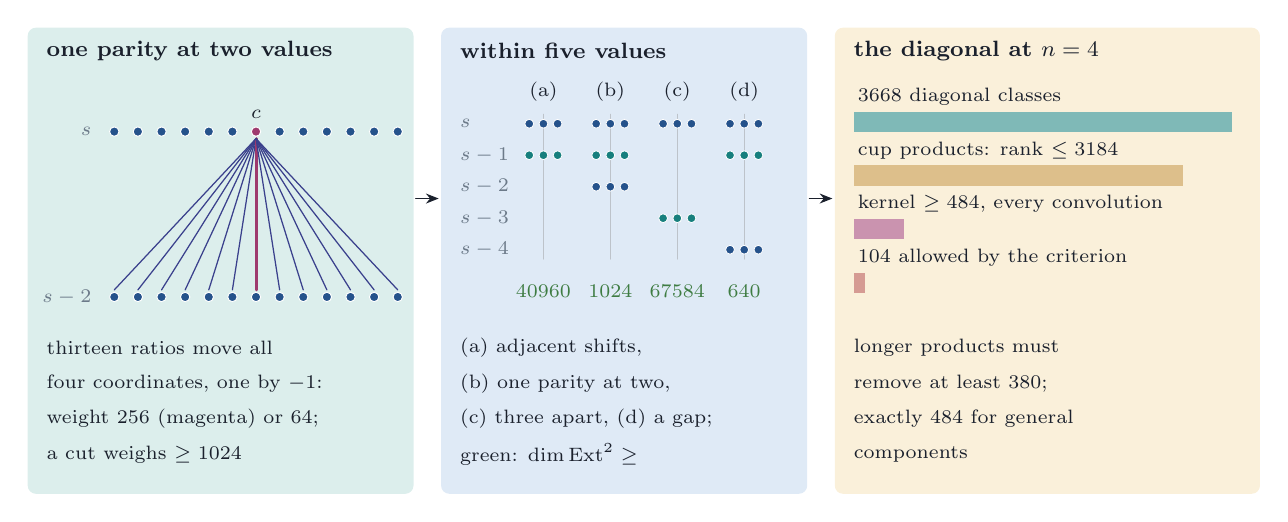
\begin{tikzpicture}[x=1cm,y=1cm,line join=round,line cap=round,
  font=\small,text=PInk,lbl/.style={inner sep=1pt}]
  \path[fill=WTeal,draw=none,rounded corners=3.0pt] (0.0500,-1.3000) rectangle (4.9500,4.6200);
  \path[fill=WBlue,draw=none,rounded corners=3.0pt] (5.3000,-1.3000) rectangle (9.9500,4.6200);
  \path[fill=WOchre,draw=none,rounded corners=3.0pt] (10.3000,-1.3000) rectangle (15.7000,4.6200);
  \path[fill=PTeal!55!white,draw=none] (10.5500,3.2900) rectangle (15.3500,3.5500);
  \path[fill=POchre!55!white,draw=none] (10.5500,2.6100) rectangle (14.7166,2.8700);
  \path[fill=PMag!55!white,draw=none] (10.5500,1.9300) rectangle (11.1834,2.1900);
  \path[fill=PClay!55!white,draw=none] (10.5500,1.2500) rectangle (10.6861,1.5100);
  \draw[PIndigo,line width=0.45pt] (2.9500,3.2100) -- (1.1500,1.2900);
  \draw[PIndigo,line width=0.45pt] (2.9500,3.2100) -- (1.4500,1.2900);
  \draw[PIndigo,line width=0.45pt] (2.9500,3.2100) -- (1.7500,1.2900);
  \draw[PIndigo,line width=0.45pt] (2.9500,3.2100) -- (2.0500,1.2900);
  \draw[PIndigo,line width=0.45pt] (2.9500,3.2100) -- (2.3500,1.2900);
  \draw[PIndigo,line width=0.45pt] (2.9500,3.2100) -- (2.6500,1.2900);
  \draw[PMag,line width=1.10pt] (2.9500,3.2100) -- (2.9500,1.2900);
  \draw[PIndigo,line width=0.45pt] (2.9500,3.2100) -- (3.2500,1.2900);
  \draw[PIndigo,line width=0.45pt] (2.9500,3.2100) -- (3.5500,1.2900);
  \draw[PIndigo,line width=0.45pt] (2.9500,3.2100) -- (3.8500,1.2900);
  \draw[PIndigo,line width=0.45pt] (2.9500,3.2100) -- (4.1500,1.2900);
  \draw[PIndigo,line width=0.45pt] (2.9500,3.2100) -- (4.4500,1.2900);
  \draw[PIndigo,line width=0.45pt] (2.9500,3.2100) -- (4.7500,1.2900);
  \path[fill=PBlue,draw=white,line width=0.35pt] (1.1500,3.3000) circle (1.70pt);
  \path[fill=PBlue,draw=white,line width=0.35pt] (1.4500,3.3000) circle (1.70pt);
  \path[fill=PBlue,draw=white,line width=0.35pt] (1.7500,3.3000) circle (1.70pt);
  \path[fill=PBlue,draw=white,line width=0.35pt] (2.0500,3.3000) circle (1.70pt);
  \path[fill=PBlue,draw=white,line width=0.35pt] (2.3500,3.3000) circle (1.70pt);
  \path[fill=PBlue,draw=white,line width=0.35pt] (2.6500,3.3000) circle (1.70pt);
  \path[fill=PMag,draw=white,line width=0.35pt] (2.9500,3.3000) circle (1.70pt);
  \path[fill=PBlue,draw=white,line width=0.35pt] (3.2500,3.3000) circle (1.70pt);
  \path[fill=PBlue,draw=white,line width=0.35pt] (3.5500,3.3000) circle (1.70pt);
  \path[fill=PBlue,draw=white,line width=0.35pt] (3.8500,3.3000) circle (1.70pt);
  \path[fill=PBlue,draw=white,line width=0.35pt] (4.1500,3.3000) circle (1.70pt);
  \path[fill=PBlue,draw=white,line width=0.35pt] (4.4500,3.3000) circle (1.70pt);
  \path[fill=PBlue,draw=white,line width=0.35pt] (4.7500,3.3000) circle (1.70pt);
  \path[fill=PBlue,draw=white,line width=0.35pt] (1.1500,1.2000) circle (1.70pt);
  \path[fill=PBlue,draw=white,line width=0.35pt] (1.4500,1.2000) circle (1.70pt);
  \path[fill=PBlue,draw=white,line width=0.35pt] (1.7500,1.2000) circle (1.70pt);
  \path[fill=PBlue,draw=white,line width=0.35pt] (2.0500,1.2000) circle (1.70pt);
  \path[fill=PBlue,draw=white,line width=0.35pt] (2.3500,1.2000) circle (1.70pt);
  \path[fill=PBlue,draw=white,line width=0.35pt] (2.6500,1.2000) circle (1.70pt);
  \path[fill=PBlue,draw=white,line width=0.35pt] (2.9500,1.2000) circle (1.70pt);
  \path[fill=PBlue,draw=white,line width=0.35pt] (3.2500,1.2000) circle (1.70pt);
  \path[fill=PBlue,draw=white,line width=0.35pt] (3.5500,1.2000) circle (1.70pt);
  \path[fill=PBlue,draw=white,line width=0.35pt] (3.8500,1.2000) circle (1.70pt);
  \path[fill=PBlue,draw=white,line width=0.35pt] (4.1500,1.2000) circle (1.70pt);
  \path[fill=PBlue,draw=white,line width=0.35pt] (4.4500,1.2000) circle (1.70pt);
  \path[fill=PBlue,draw=white,line width=0.35pt] (4.7500,1.2000) circle (1.70pt);
  \draw[PSlate!45!white,line width=0.4pt] (6.6000,3.5200) -- (6.6000,1.6800);
  \path[fill=PBlue,draw=white,line width=0.30pt] (6.4200,3.4000) circle (1.60pt);
  \path[fill=PBlue,draw=white,line width=0.30pt] (6.6000,3.4000) circle (1.60pt);
  \path[fill=PBlue,draw=white,line width=0.30pt] (6.7800,3.4000) circle (1.60pt);
  \path[fill=PTeal,draw=white,line width=0.30pt] (6.4200,3.0000) circle (1.60pt);
  \path[fill=PTeal,draw=white,line width=0.30pt] (6.6000,3.0000) circle (1.60pt);
  \path[fill=PTeal,draw=white,line width=0.30pt] (6.7800,3.0000) circle (1.60pt);
  \draw[PSlate!45!white,line width=0.4pt] (7.4500,3.5200) -- (7.4500,1.6800);
  \path[fill=PBlue,draw=white,line width=0.30pt] (7.2700,3.4000) circle (1.60pt);
  \path[fill=PBlue,draw=white,line width=0.30pt] (7.4500,3.4000) circle (1.60pt);
  \path[fill=PBlue,draw=white,line width=0.30pt] (7.6300,3.4000) circle (1.60pt);
  \path[fill=PBlue,draw=white,line width=0.30pt] (7.2700,2.6000) circle (1.60pt);
  \path[fill=PBlue,draw=white,line width=0.30pt] (7.4500,2.6000) circle (1.60pt);
  \path[fill=PBlue,draw=white,line width=0.30pt] (7.6300,2.6000) circle (1.60pt);
  \path[fill=PTeal,draw=white,line width=0.30pt] (7.2700,3.0000) circle (1.60pt);
  \path[fill=PTeal,draw=white,line width=0.30pt] (7.4500,3.0000) circle (1.60pt);
  \path[fill=PTeal,draw=white,line width=0.30pt] (7.6300,3.0000) circle (1.60pt);
  \draw[PSlate!45!white,line width=0.4pt] (8.3000,3.5200) -- (8.3000,1.6800);
  \path[fill=PBlue,draw=white,line width=0.30pt] (8.1200,3.4000) circle (1.60pt);
  \path[fill=PBlue,draw=white,line width=0.30pt] (8.3000,3.4000) circle (1.60pt);
  \path[fill=PBlue,draw=white,line width=0.30pt] (8.4800,3.4000) circle (1.60pt);
  \path[fill=PTeal,draw=white,line width=0.30pt] (8.1200,2.2000) circle (1.60pt);
  \path[fill=PTeal,draw=white,line width=0.30pt] (8.3000,2.2000) circle (1.60pt);
  \path[fill=PTeal,draw=white,line width=0.30pt] (8.4800,2.2000) circle (1.60pt);
  \draw[PSlate!45!white,line width=0.4pt] (9.1500,3.5200) -- (9.1500,1.6800);
  \path[fill=PBlue,draw=white,line width=0.30pt] (8.9700,3.4000) circle (1.60pt);
  \path[fill=PBlue,draw=white,line width=0.30pt] (9.1500,3.4000) circle (1.60pt);
  \path[fill=PBlue,draw=white,line width=0.30pt] (9.3300,3.4000) circle (1.60pt);
  \path[fill=PBlue,draw=white,line width=0.30pt] (8.9700,1.8000) circle (1.60pt);
  \path[fill=PBlue,draw=white,line width=0.30pt] (9.1500,1.8000) circle (1.60pt);
  \path[fill=PBlue,draw=white,line width=0.30pt] (9.3300,1.8000) circle (1.60pt);
  \path[fill=PTeal,draw=white,line width=0.30pt] (8.9700,3.0000) circle (1.60pt);
  \path[fill=PTeal,draw=white,line width=0.30pt] (9.1500,3.0000) circle (1.60pt);
  \path[fill=PTeal,draw=white,line width=0.30pt] (9.3300,3.0000) circle (1.60pt);
  \draw[PInk,line width=0.6pt,-{Stealth[length=4.6pt,width=3.6pt]}] (4.9800,2.4500) -- (5.2700,2.4500);
  \draw[PInk,line width=0.6pt,-{Stealth[length=4.6pt,width=3.6pt]}] (9.9800,2.4500) -- (10.2700,2.4500);
  \node[lbl,anchor=west,text=PInk,font=\footnotesize] at (0.2500,4.3200) {\textbf{one parity at two values}};
  \node[lbl,anchor=east,text=PSlate,font=\scriptsize] at (0.9000,3.3000) {$s$};
  \node[lbl,anchor=east,text=PSlate,font=\scriptsize] at (0.9000,1.2000) {$s-2$};
  \node[lbl,anchor=south,text=PInk,font=\scriptsize] at (2.9500,3.4300) {$c$};
  \node[lbl,anchor=west,text=PInk,font=\scriptsize] at (0.2500,0.5500) {thirteen ratios move all};
  \node[lbl,anchor=west,text=PInk,font=\scriptsize] at (0.2500,0.1000) {four coordinates, one by $-1$:};
  \node[lbl,anchor=west,text=PInk,font=\scriptsize] at (0.2500,-0.3500) {weight $256$ (magenta) or $64$;};
  \node[lbl,anchor=west,text=PInk,font=\scriptsize] at (0.2500,-0.8000) {a cut weighs $\ge1024$};
  \node[lbl,anchor=west,text=PInk,font=\footnotesize] at (5.5000,4.3200) {\textbf{within five values}};
  \node[lbl,anchor=west,text=PSlate,font=\scriptsize] at (5.5000,3.4000) {$s$};
  \node[lbl,anchor=west,text=PSlate,font=\scriptsize] at (5.5000,3.0000) {$s-1$};
  \node[lbl,anchor=west,text=PSlate,font=\scriptsize] at (5.5000,2.6000) {$s-2$};
  \node[lbl,anchor=west,text=PSlate,font=\scriptsize] at (5.5000,2.2000) {$s-3$};
  \node[lbl,anchor=west,text=PSlate,font=\scriptsize] at (5.5000,1.8000) {$s-4$};
  \node[lbl,anchor=south,text=PInk,font=\scriptsize] at (6.6000,3.6400) {(a)};
  \node[lbl,anchor=south,text=PInk,font=\scriptsize] at (7.4500,3.6400) {(b)};
  \node[lbl,anchor=south,text=PInk,font=\scriptsize] at (8.3000,3.6400) {(c)};
  \node[lbl,anchor=south,text=PInk,font=\scriptsize] at (9.1500,3.6400) {(d)};
  \node[lbl,anchor=north,text=PGrass,font=\scriptsize] at (6.6000,1.4000) {$40960$};
  \node[lbl,anchor=north,text=PGrass,font=\scriptsize] at (7.4500,1.4000) {$1024$};
  \node[lbl,anchor=north,text=PGrass,font=\scriptsize] at (8.3000,1.4000) {$67584$};
  \node[lbl,anchor=north,text=PGrass,font=\scriptsize] at (9.1500,1.4000) {$640$};
  \node[lbl,anchor=west,text=PInk,font=\scriptsize] at (5.5000,0.5500) {(a) adjacent shifts,};
  \node[lbl,anchor=west,text=PInk,font=\scriptsize] at (5.5000,0.1000) {(b) one parity at two,};
  \node[lbl,anchor=west,text=PInk,font=\scriptsize] at (5.5000,-0.3500) {(c) three apart, (d) a gap;};
  \node[lbl,anchor=west,text=PInk,font=\scriptsize] at (5.5000,-0.8000) {green: $\dim\Ext^{2}\ge$};
  \node[lbl,anchor=west,text=PInk,font=\footnotesize] at (10.5000,4.3200) {\textbf{the diagonal at $n=4$}};
  \node[lbl,anchor=west,text=PInk,font=\scriptsize] at (10.5500,3.7415) {$3668$ diagonal classes};
  \node[lbl,anchor=west,text=PInk,font=\scriptsize] at (10.5500,3.0615) {cup products: rank $\le3184$};
  \node[lbl,anchor=west,text=PInk,font=\scriptsize] at (10.5500,2.3815) {kernel $\ge484$, every convolution};
  \node[lbl,anchor=west,text=PInk,font=\scriptsize] at (10.5500,1.7015) {$104$ allowed by the criterion};
  \node[lbl,anchor=west,text=PInk,font=\scriptsize] at (10.5000,0.5500) {longer products must};
  \node[lbl,anchor=west,text=PInk,font=\scriptsize] at (10.5000,0.1000) {remove at least $380$;};
  \node[lbl,anchor=west,text=PInk,font=\scriptsize] at (10.5000,-0.3500) {exactly $484$ for general};
  \node[lbl,anchor=west,text=PInk,font=\scriptsize] at (10.5000,-0.8000) {components};
\end{tikzpicture}
\end{document}
